\documentclass[english,compress]{beamer}

\usepackage{listings}
\useoutertheme{split}
\useinnertheme{rectangles}
\usecolortheme{uiuc}
\logo{
\includegraphics[height=0.5cm]{uiuclogo.pdf}}

\title{SIAM: Getting Started with Git}
\subtitle{based on http://git-scm.com/book}
\author{Andrew Reisner}
\date{\today}

\begin{document}
\nocite{*}
\frame{\titlepage}

\frame
{
    \frametitle{Overview}
    \begin{columns}
    \begin{column}{.5\textwidth}
        Git is a
        \begin{itemize}
            \item Free and Open Source
            \item Distributed
            \item Version Control System.
        \end{itemize}
    \end{column}
    \begin{column}{.5\textwidth}
        \begin{center}
            
\includegraphics[width=.7\textwidth]{figs/git-logo.png} 
        \end{center}
    \end{column}
    \end{columns}
}

\frame
{
    \frametitle{Version Control System}
    \begin{columns}
    \begin{column}{.7\textwidth}
    \begin{itemize}
        \item Record changes to files
        \item Versions can be recalled later
        \item Terminology
        \begin{itemize}
            \item Repository
            \item Working copy
            \item Checkout
            \item Commit
            \item Branch
            \item Merge
        \end{itemize}
    \end{itemize}
    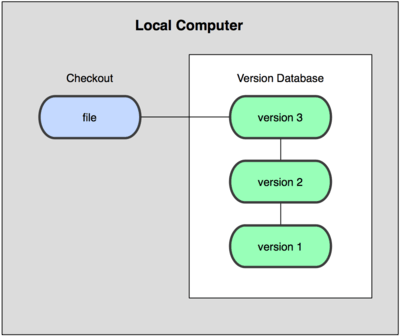
\includegraphics[width=.5\textwidth]{figs/vc.png}
    \end{column}
    \begin{column}{.3\textwidth}
    \begin{center}
    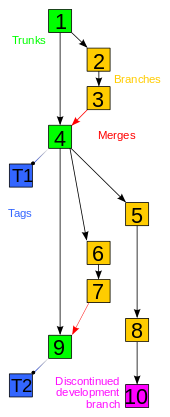
\includegraphics[width=.8\textwidth]{figs/vc-graph.png}
    \end{center}
    \end{column}
    \end{columns}
}

\frame
{
    \frametitle{Version Control System}
    \begin{columns}
    \begin{column}{.6\textwidth}
        \begin{itemize}
            \item Local repository: directory containing a collection of commits and metadata for a project
            \item Staging area (Index): file detailing content of next commit, allows for incrementally building commits
            \item Working directory: single checkout of one version of the project
        \end{itemize}
    \end{column}
    \begin{column}{.4\textwidth}
        \begin{center}
            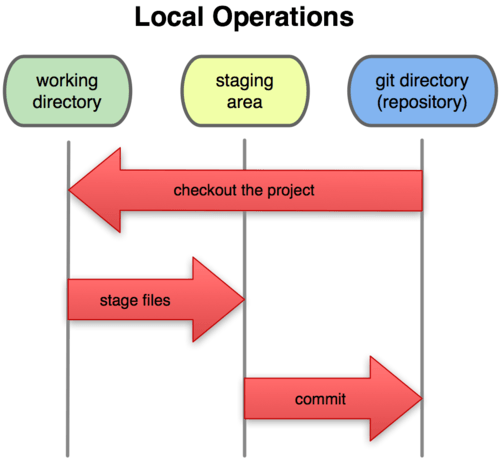
\includegraphics[width=.8\textwidth]{figs/sections.png}
        \end{center}
        \end{column}
    \end{columns}
}

\frame
{
    \frametitle{Distributed}
    \begin{itemize}
        \item No central location that keeps trakc of your data (no single place is more important than another)
        \item Encourages small commits and frequent merging
        \item Branches don't affect the main repository and can commit changes without disturbing others
        \item Work offline
        \item Rely on a network of trust
    \end{itemize}
}

\frame
{
    \frametitle{Distributed Workflows: Centralized}

    \begin{center}
        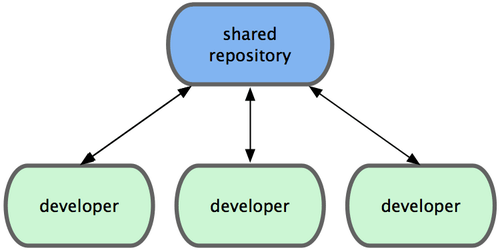
\includegraphics[width=.7\textwidth]{figs/centralized-workflow.png}
    \end{center}
}

\frame
{
    \frametitle{Distributed Workflows: Integration-Manager}

    \begin{center}
        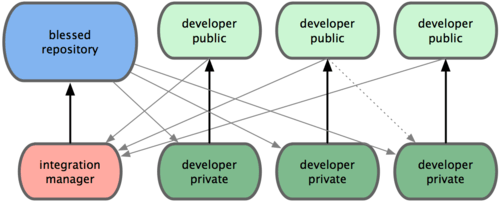
\includegraphics[width=.7\textwidth]{figs/integration-manager-workflow.png}
    \end{center}

}

\frame
{
    \frametitle{Distributed Workflows: Dictator and Lieutenants}

    \begin{center}
        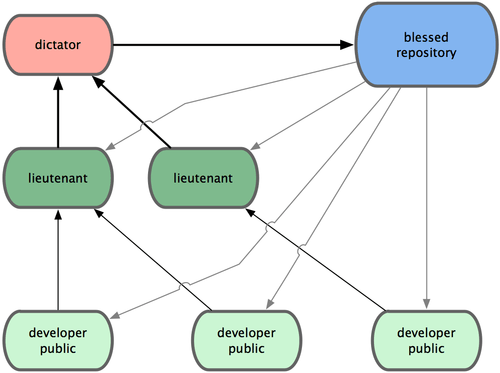
\includegraphics[width=.7\textwidth]{figs/dictator-lieutenant-workflow.png}
    \end{center}

}

\frame
{
    \frametitle{Free and Open Source}

    \begin{itemize}
        \item Downloads at \url{http://git-scm.com}
        \item Libgit2: free and open source library for writing custom Git applications
        \begin{columns}
            \begin{column}{.5\textwidth}
                \begin{center}
                    
\includegraphics[width=1\textwidth]{figs/git-logo1.png}
                \end{center}
            \end{column}
            \begin{column}{.5\textwidth}
                \begin{center}
                    
\includegraphics[width=1\textwidth]{figs/libgit-logo.png}
                \end{center}
            \end{column}
        \end{columns}
    \end{itemize}
}

\frame
{
    \frametitle{GitHub}

}


\frame
{
\small
    \frametitle{Resources}
    \begin{enumerate}
        \item Git From the Bottom Up\\
            \url{http://ftp.newartisans.com/pub/git.from.bottom.up.pdf}
        \item User Manual\\
            \url{http://git-scm.com/docs/user-manual.html}
        \item Git Magic\\
            \url{http://www-cs-students.stanford.edu/~blynn/gitmagic/}
        \item Git Book\\
            \url{http://git-scm.com/book}
        \item Tech Talk: Linus Torvalds on git\\
            \url{http://youtu.be/4XpnKHJAok8} 
        \item Code School - Try Git\\
            \url{http://try.github.io}
    \end{enumerate}
}
\end{document}
